\chapter[Supplementaries for \citet{varoquaux:accurate}]{Supplementary information for
\citet{varoquaux:accurate}}
\label{chap:centurion_supp}

\graphicspath{{9_centurion_supplementaries/}}


\begin{figure}[ht!]
\caption{\textbf{Error on centromere calls for \textit{P. falciparum} on raw
and normalized contact counts (40~kb)}}{
\textbf{A.} ring stage \textbf{B.}
trophozoite stage \textbf{C.} schizont stage}
\begin{center}
\includegraphics[width=0.7\linewidth]{figures/supp/supp_2.pdf}
\end{center}
\label{suppfig:raw_vs_normed_pf}
\end{figure}

\clearpage

\begin{figure}[ht!]
\caption{\textbf{Error on centromere calls for \textit{S. cerevisiae}
at different resolutions (10~kb, 20~kb, 40~kb)}}
\begin{center}
\includegraphics[width=0.8\linewidth]{figures/supp/pf_different_resolution_duan.SC.pdf}
\end{center}
\label{suppfig:error_diff_res_sc}
\end{figure}


\begin{figure}[ht!]
\caption{\textbf{Error on centromere calls for \textit{P. falciparum}
at different resolutions (10~kb, 20~kb, 40~kb)}}
{\textbf{A.} ring stage \textbf{B.} trophozoite stage \textbf{C.} schizont stage}
\begin{center}
\includegraphics[width=0.8\linewidth]{figures/supp/supp_4.pdf}
\end{center}
\label{suppfig:error_diff_res_pf}
\end{figure}

\clearpage

\begin{table}[ht!]
\caption{\textbf{Centromere calls for \textit{S. cerevisiae}, ground truth and
errors}}
\vspace{10pt}
\small
\begin{center}
\begin{tabular}{c | c  r  r  r  r r r}
\textbf{Chromosome}  & \textbf{Ground truth} & \multicolumn{2}{c}{\textbf{10~kb}} & \multicolumn{2}{c}{\textbf{20~kb}} & \multicolumn{2}{c}{\textbf{40~kb}} \\
  &   &  \multicolumn{1}{c}{\textbf{Call}} &  \multicolumn{1}{c}{\textbf{Error}} &  \multicolumn{1}{c}{\textbf{Call}} &  \multicolumn{1}{c}{\textbf{Error}} &  \multicolumn{1}{c}{\textbf{Call}} &  \multicolumn{1}{c}{\textbf{Error}} \\
\hline
I & \num[group-separator={\,}]{151584} - \num[group-separator={\,}]{151584} & \num[group-separator={\,}]{153319} & \small{\num[group-separator={\,}]{1735}}  & \num[group-separator={\,}]{154614} & \small{\num[group-separator={\,}]{3030}}  & \num[group-separator={\,}]{153633} & \small{\num[group-separator={\,}]{2049}}  \\
II & \num[group-separator={\,}]{238325} - \num[group-separator={\,}]{238325} & \num[group-separator={\,}]{238994} & \small{\num[group-separator={\,}]{669}}  & \num[group-separator={\,}]{237386} & \small{\num[group-separator={\,}]{939}}  & \num[group-separator={\,}]{236883} & \small{\num[group-separator={\,}]{1442}}  \\
III & \num[group-separator={\,}]{114499} - \num[group-separator={\,}]{114499} & \num[group-separator={\,}]{108309} & \small{\num[group-separator={\,}]{6190}}  & \num[group-separator={\,}]{110914} & \small{\num[group-separator={\,}]{3585}}  & \num[group-separator={\,}]{109488} & \small{\num[group-separator={\,}]{5011}}  \\
IV & \num[group-separator={\,}]{449819} - \num[group-separator={\,}]{449819} & \num[group-separator={\,}]{451567} & \small{\num[group-separator={\,}]{1748}}  & \num[group-separator={\,}]{450459} & \small{\num[group-separator={\,}]{640}}  & \num[group-separator={\,}]{452579} & \small{\num[group-separator={\,}]{2760}}  \\
V & \num[group-separator={\,}]{152103} - \num[group-separator={\,}]{152103} & \num[group-separator={\,}]{155434} & \small{\num[group-separator={\,}]{3331}}  & \num[group-separator={\,}]{149350} & \small{\num[group-separator={\,}]{2753}}  & \num[group-separator={\,}]{152162} & \small{\num[group-separator={\,}]{59}}  \\
VI & \num[group-separator={\,}]{148622} - \num[group-separator={\,}]{148622} & \num[group-separator={\,}]{150691} & \small{\num[group-separator={\,}]{2069}}  & \num[group-separator={\,}]{149718} & \small{\num[group-separator={\,}]{1096}}  & \num[group-separator={\,}]{148387} & \small{\num[group-separator={\,}]{235}}  \\
VII & \num[group-separator={\,}]{497042} - \num[group-separator={\,}]{497042} & \num[group-separator={\,}]{499561} & \small{\num[group-separator={\,}]{2519}}  & \num[group-separator={\,}]{501816} & \small{\num[group-separator={\,}]{4774}}  & \num[group-separator={\,}]{502369} & \small{\num[group-separator={\,}]{5327}}  \\
VIII & \num[group-separator={\,}]{105698} - \num[group-separator={\,}]{105698} & \num[group-separator={\,}]{102152} & \small{\num[group-separator={\,}]{3546}}  & \num[group-separator={\,}]{101652} & \small{\num[group-separator={\,}]{4046}}  & \num[group-separator={\,}]{101007} & \small{\num[group-separator={\,}]{4691}}  \\
IX & \num[group-separator={\,}]{355742} - \num[group-separator={\,}]{355742} & \num[group-separator={\,}]{364818} & \small{\num[group-separator={\,}]{9076}}  & \num[group-separator={\,}]{361667} & \small{\num[group-separator={\,}]{5925}}  & \num[group-separator={\,}]{355631} & \small{\num[group-separator={\,}]{111}}  \\
X & \num[group-separator={\,}]{436418} - \num[group-separator={\,}]{436418} & \num[group-separator={\,}]{436467} & \small{\num[group-separator={\,}]{49}}  & \num[group-separator={\,}]{435999} & \small{\num[group-separator={\,}]{419}}  & \num[group-separator={\,}]{437603} & \small{\num[group-separator={\,}]{1185}}  \\
XI & \num[group-separator={\,}]{439889} - \num[group-separator={\,}]{439889} & \num[group-separator={\,}]{444216} & \small{\num[group-separator={\,}]{4327}}  & \num[group-separator={\,}]{446174} & \small{\num[group-separator={\,}]{6285}}  & \num[group-separator={\,}]{444533} & \small{\num[group-separator={\,}]{4644}}  \\
XII & \num[group-separator={\,}]{150946} - \num[group-separator={\,}]{150946} & \num[group-separator={\,}]{149704} & \small{\num[group-separator={\,}]{1242}}  & \num[group-separator={\,}]{147393} & \small{\num[group-separator={\,}]{3553}}  & \num[group-separator={\,}]{144489} & \small{\num[group-separator={\,}]{6457}}  \\
XIII & \num[group-separator={\,}]{268149} - \num[group-separator={\,}]{268149} & \num[group-separator={\,}]{264502} & \small{\num[group-separator={\,}]{3647}}  & \num[group-separator={\,}]{266704} & \small{\num[group-separator={\,}]{1445}}  & \num[group-separator={\,}]{267860} & \small{\num[group-separator={\,}]{289}}  \\
XIV & \num[group-separator={\,}]{628877} - \num[group-separator={\,}]{628877} & \num[group-separator={\,}]{629542} & \small{\num[group-separator={\,}]{665}}  & \num[group-separator={\,}]{629178} & \small{\num[group-separator={\,}]{301}}  & \num[group-separator={\,}]{627374} & \small{\num[group-separator={\,}]{1503}}  \\
XV & \num[group-separator={\,}]{326703} - \num[group-separator={\,}]{326703} & \num[group-separator={\,}]{327448} & \small{\num[group-separator={\,}]{745}}  & \num[group-separator={\,}]{328019} & \small{\num[group-separator={\,}]{1316}}  & \num[group-separator={\,}]{326866} & \small{\num[group-separator={\,}]{163}}  \\
XVI & \num[group-separator={\,}]{556070} - \num[group-separator={\,}]{556070} & \num[group-separator={\,}]{553705} & \small{\num[group-separator={\,}]{2365}}  & \num[group-separator={\,}]{555162} & \small{\num[group-separator={\,}]{908}}  & \num[group-separator={\,}]{554062} & \small{\num[group-separator={\,}]{2008}}  \\
\end{tabular}
\end{center}
\label{supptable:sc_results}
\end{table}



\clearpage


\begin{table}[ht!]
\caption{\textbf{Centromere calls for \textit{P. falciparum} (ring stage),
ground truth and errors}}
\small
\vspace{10pt}
\begin{center}
\begin{tabular}{c | c  r  r  r  r r r}
\textbf{Chromosome}  & \textbf{Ground truth} & \multicolumn{2}{c}{\textbf{10~kb}} & \multicolumn{2}{c}{\textbf{20~kb}} & \multicolumn{2}{c}{\textbf{40~kb}} \\
  &   &  \multicolumn{1}{c}{\textbf{Call}} &  \multicolumn{1}{c}{\textbf{Error}} &  \multicolumn{1}{c}{\textbf{Call}} &  \multicolumn{1}{c}{\textbf{Error}} &  \multicolumn{1}{c}{\textbf{Call}} &  \multicolumn{1}{c}{\textbf{Error}} \\
\hline
I & \num[group-separator={\,}]{456871} - \num[group-separator={\,}]{461511} & \num[group-separator={\,}]{458108} & \small{\num[group-separator={\,}]{0}}  & \num[group-separator={\,}]{457710} & \small{\num[group-separator={\,}]{0}}  & \num[group-separator={\,}]{455394} & \small{\num[group-separator={\,}]{1477}}  \\
II & \num[group-separator={\,}]{446771} - \num[group-separator={\,}]{450941} & \num[group-separator={\,}]{448688} & \small{\num[group-separator={\,}]{0}}  & \num[group-separator={\,}]{448953} & \small{\num[group-separator={\,}]{0}}  & \num[group-separator={\,}]{452647} & \small{\num[group-separator={\,}]{1706}}  \\
III & \num[group-separator={\,}]{597014} - \num[group-separator={\,}]{601275} & \num[group-separator={\,}]{599187} & \small{\num[group-separator={\,}]{0}}  & \num[group-separator={\,}]{597486} & \small{\num[group-separator={\,}]{0}}  & \num[group-separator={\,}]{599779} & \small{\num[group-separator={\,}]{0}}  \\
IV & \num[group-separator={\,}]{641019} - \num[group-separator={\,}]{645339} & \num[group-separator={\,}]{644178} & \small{\num[group-separator={\,}]{0}}  & \num[group-separator={\,}]{644931} & \small{\num[group-separator={\,}]{0}}  & \num[group-separator={\,}]{648176} & \small{\num[group-separator={\,}]{2837}}  \\
V & \num[group-separator={\,}]{454543} - \num[group-separator={\,}]{458793} & \num[group-separator={\,}]{456329} & \small{\num[group-separator={\,}]{0}}  & \num[group-separator={\,}]{455929} & \small{\num[group-separator={\,}]{0}}  & \num[group-separator={\,}]{454201} & \small{\num[group-separator={\,}]{342}}  \\
VI & \num[group-separator={\,}]{477756} - \num[group-separator={\,}]{482016} & \num[group-separator={\,}]{480602} & \small{\num[group-separator={\,}]{0}}  & \num[group-separator={\,}]{477287} & \small{\num[group-separator={\,}]{469}}  & \num[group-separator={\,}]{482950} & \small{\num[group-separator={\,}]{934}}  \\
VII & \num[group-separator={\,}]{808365} - \num[group-separator={\,}]{812875} & \num[group-separator={\,}]{811744} & \small{\num[group-separator={\,}]{0}}  & \num[group-separator={\,}]{810236} & \small{\num[group-separator={\,}]{0}}  & \num[group-separator={\,}]{812304} & \small{\num[group-separator={\,}]{0}}  \\
VIII & \num[group-separator={\,}]{297895} - \num[group-separator={\,}]{302515} & \num[group-separator={\,}]{299983} & \small{\num[group-separator={\,}]{0}}  & \num[group-separator={\,}]{297460} & \small{\num[group-separator={\,}]{435}}  & \num[group-separator={\,}]{297824} & \small{\num[group-separator={\,}]{71}}  \\
IX & \num[group-separator={\,}]{1241081} - \num[group-separator={\,}]{1245451} & \num[group-separator={\,}]{1242788} & \small{\num[group-separator={\,}]{0}}  & \num[group-separator={\,}]{1242570} & \small{\num[group-separator={\,}]{0}}  & \num[group-separator={\,}]{1247435} & \small{\num[group-separator={\,}]{1984}}  \\
X & \num[group-separator={\,}]{935682} - \num[group-separator={\,}]{937823} & \num[group-separator={\,}]{937162} & \small{\num[group-separator={\,}]{0}}  & \num[group-separator={\,}]{936247} & \small{\num[group-separator={\,}]{0}}  & \num[group-separator={\,}]{938213} & \small{\num[group-separator={\,}]{390}}  \\
XI & \num[group-separator={\,}]{830782} - \num[group-separator={\,}]{835432} & \num[group-separator={\,}]{832728} & \small{\num[group-separator={\,}]{0}}  & \num[group-separator={\,}]{832858} & \small{\num[group-separator={\,}]{0}}  & \num[group-separator={\,}]{834051} & \small{\num[group-separator={\,}]{0}}  \\
XII & \num[group-separator={\,}]{1281521} - \num[group-separator={\,}]{1285941} & \num[group-separator={\,}]{1284567} & \small{\num[group-separator={\,}]{0}}  & \num[group-separator={\,}]{1285214} & \small{\num[group-separator={\,}]{0}}  & \num[group-separator={\,}]{1285943} & \small{\num[group-separator={\,}]{2}}  \\
XIII & \num[group-separator={\,}]{1167070} - \num[group-separator={\,}]{1171720} & \num[group-separator={\,}]{1166999} & \small{\num[group-separator={\,}]{71}}  & \num[group-separator={\,}]{1168375} & \small{\num[group-separator={\,}]{0}}  & \num[group-separator={\,}]{1172174} & \small{\num[group-separator={\,}]{454}}  \\
XIV & \num[group-separator={\,}]{1070909} - \num[group-separator={\,}]{1075369} & \num[group-separator={\,}]{1072595} & \small{\num[group-separator={\,}]{0}}  & \num[group-separator={\,}]{1072131} & \small{\num[group-separator={\,}]{0}}  & \num[group-separator={\,}]{1069179} & \small{\num[group-separator={\,}]{1730}}  \\
\end{tabular}
\end{center}
\label{supptable:rings_results}
\end{table}

\clearpage

\begin{table}[ht!]
\caption{\textbf{Centromere calls for \textit{P. falciparum} (trophozoite stage),
ground truth and errors}}
\small
\vspace{10pt}
\begin{center}
\begin{tabular}{c | c  r  r  r  r r r}
\textbf{Chromosome}  & \textbf{Ground truth} & \multicolumn{2}{c}{\textbf{10~kb}} & \multicolumn{2}{c}{\textbf{20~kb}} & \multicolumn{2}{c}{\textbf{40~kb}} \\
  &   &  \multicolumn{1}{c}{\textbf{Call}} &  \multicolumn{1}{c}{\textbf{Error}} &  \multicolumn{1}{c}{\textbf{Call}} &  \multicolumn{1}{c}{\textbf{Error}} &  \multicolumn{1}{c}{\textbf{Call}} &  \multicolumn{1}{c}{\textbf{Error}} \\
\hline
I & \num[group-separator={\,}]{456871} - \num[group-separator={\,}]{461511} & \num[group-separator={\,}]{456134} & \small{\num[group-separator={\,}]{737}}  & \num[group-separator={\,}]{454096} & \small{\num[group-separator={\,}]{2775}}  & \num[group-separator={\,}]{450980} & \small{\num[group-separator={\,}]{5891}}  \\
II & \num[group-separator={\,}]{446771} - \num[group-separator={\,}]{450941} & \num[group-separator={\,}]{448623} & \small{\num[group-separator={\,}]{0}}  & \num[group-separator={\,}]{447562} & \small{\num[group-separator={\,}]{0}}  & \num[group-separator={\,}]{448953} & \small{\num[group-separator={\,}]{0}}  \\
III & \num[group-separator={\,}]{597014} - \num[group-separator={\,}]{601275} & \num[group-separator={\,}]{598035} & \small{\num[group-separator={\,}]{0}}  & \num[group-separator={\,}]{597348} & \small{\num[group-separator={\,}]{0}}  & \num[group-separator={\,}]{597426} & \small{\num[group-separator={\,}]{0}}  \\
IV & \num[group-separator={\,}]{641019} - \num[group-separator={\,}]{645339} & \num[group-separator={\,}]{645248} & \small{\num[group-separator={\,}]{0}}  & \num[group-separator={\,}]{647059} & \small{\num[group-separator={\,}]{1720}}  & \num[group-separator={\,}]{654977} & \small{\num[group-separator={\,}]{9638}}  \\
V & \num[group-separator={\,}]{454543} - \num[group-separator={\,}]{458793} & \num[group-separator={\,}]{455899} & \small{\num[group-separator={\,}]{0}}  & \num[group-separator={\,}]{455305} & \small{\num[group-separator={\,}]{0}}  & \num[group-separator={\,}]{457291} & \small{\num[group-separator={\,}]{0}}  \\
VI & \num[group-separator={\,}]{477756} - \num[group-separator={\,}]{482016} & \num[group-separator={\,}]{480552} & \small{\num[group-separator={\,}]{0}}  & \num[group-separator={\,}]{477010} & \small{\num[group-separator={\,}]{746}}  & \num[group-separator={\,}]{480417} & \small{\num[group-separator={\,}]{0}}  \\
VII & \num[group-separator={\,}]{808365} - \num[group-separator={\,}]{812875} & \num[group-separator={\,}]{810348} & \small{\num[group-separator={\,}]{0}}  & \num[group-separator={\,}]{807779} & \small{\num[group-separator={\,}]{586}}  & \num[group-separator={\,}]{807937} & \small{\num[group-separator={\,}]{428}}  \\
VIII & \num[group-separator={\,}]{297895} - \num[group-separator={\,}]{302515} & \num[group-separator={\,}]{297355} & \small{\num[group-separator={\,}]{540}}  & \num[group-separator={\,}]{292808} & \small{\num[group-separator={\,}]{5087}}  & \num[group-separator={\,}]{293495} & \small{\num[group-separator={\,}]{4400}}  \\
IX & \num[group-separator={\,}]{1241081} - \num[group-separator={\,}]{1245451} & \num[group-separator={\,}]{1240449} & \small{\num[group-separator={\,}]{632}}  & \num[group-separator={\,}]{1238687} & \small{\num[group-separator={\,}]{2394}}  & \num[group-separator={\,}]{1239714} & \small{\num[group-separator={\,}]{1367}}  \\
X & \num[group-separator={\,}]{935682} - \num[group-separator={\,}]{937823} & \num[group-separator={\,}]{936765} & \small{\num[group-separator={\,}]{0}}  & \num[group-separator={\,}]{938559} & \small{\num[group-separator={\,}]{736}}  & \num[group-separator={\,}]{937531} & \small{\num[group-separator={\,}]{0}}  \\
XI & \num[group-separator={\,}]{830782} - \num[group-separator={\,}]{835432} & \num[group-separator={\,}]{832425} & \small{\num[group-separator={\,}]{0}}  & \num[group-separator={\,}]{833938} & \small{\num[group-separator={\,}]{0}}  & \num[group-separator={\,}]{833994} & \small{\num[group-separator={\,}]{0}}  \\
XII & \num[group-separator={\,}]{1281521} - \num[group-separator={\,}]{1285941} & \num[group-separator={\,}]{1284634} & \small{\num[group-separator={\,}]{0}}  & \num[group-separator={\,}]{1284403} & \small{\num[group-separator={\,}]{0}}  & \num[group-separator={\,}]{1282674} & \small{\num[group-separator={\,}]{0}}  \\
XIII & \num[group-separator={\,}]{1167070} - \num[group-separator={\,}]{1171720} & \num[group-separator={\,}]{1168647} & \small{\num[group-separator={\,}]{0}}  & \num[group-separator={\,}]{1168225} & \small{\num[group-separator={\,}]{0}}  & \num[group-separator={\,}]{1166916} & \small{\num[group-separator={\,}]{154}}  \\
XIV & \num[group-separator={\,}]{1070909} - \num[group-separator={\,}]{1075369} & \num[group-separator={\,}]{1071170} & \small{\num[group-separator={\,}]{0}}  & \num[group-separator={\,}]{1069381} & \small{\num[group-separator={\,}]{1528}}  & \num[group-separator={\,}]{1065476} & \small{\num[group-separator={\,}]{5433}}  \\
\end{tabular}
\end{center}
\label{supptable:trophs_results}
\end{table}

\clearpage

\begin{table}[ht!]
\caption{\textbf{Centromere calls for \textit{P. falciparum} (schizont stage),
ground truth and errors}}
\vspace{10pt}
\small
\begin{center}
\begin{tabular}{c | c  r  r  r  r r r}
\textbf{Chromosome}  & \textbf{Ground truth} & \multicolumn{2}{c}{\textbf{10~kb}} & \multicolumn{2}{c}{\textbf{20~kb}} & \multicolumn{2}{c}{\textbf{40~kb}} \\
  &   &  \multicolumn{1}{c}{\textbf{Call}} &  \multicolumn{1}{c}{\textbf{Error}} &  \multicolumn{1}{c}{\textbf{Call}} &  \multicolumn{1}{c}{\textbf{Error}} &  \multicolumn{1}{c}{\textbf{Call}} &  \multicolumn{1}{c}{\textbf{Error}} \\
\hline
I & \num[group-separator={\,}]{456871} - \num[group-separator={\,}]{461511} & \num[group-separator={\,}]{458269} & \small{\num[group-separator={\,}]{0}}  & \num[group-separator={\,}]{456457} & \small{\num[group-separator={\,}]{414}}  & \num[group-separator={\,}]{453275} & \small{\num[group-separator={\,}]{3596}}  \\
II & \num[group-separator={\,}]{446771} - \num[group-separator={\,}]{450941} & \num[group-separator={\,}]{448913} & \small{\num[group-separator={\,}]{0}}  & \num[group-separator={\,}]{448374} & \small{\num[group-separator={\,}]{0}}  & \num[group-separator={\,}]{450640} & \small{\num[group-separator={\,}]{0}}  \\
III & \num[group-separator={\,}]{597014} - \num[group-separator={\,}]{601275} & \num[group-separator={\,}]{599091} & \small{\num[group-separator={\,}]{0}}  & \num[group-separator={\,}]{597694} & \small{\num[group-separator={\,}]{0}}  & \num[group-separator={\,}]{598616} & \small{\num[group-separator={\,}]{0}}  \\
IV & \num[group-separator={\,}]{641019} - \num[group-separator={\,}]{645339} & \num[group-separator={\,}]{644640} & \small{\num[group-separator={\,}]{0}}  & \num[group-separator={\,}]{646085} & \small{\num[group-separator={\,}]{746}}  & \num[group-separator={\,}]{651741} & \small{\num[group-separator={\,}]{6402}}  \\
V & \num[group-separator={\,}]{454543} - \num[group-separator={\,}]{458793} & \num[group-separator={\,}]{455379} & \small{\num[group-separator={\,}]{0}}  & \num[group-separator={\,}]{454880} & \small{\num[group-separator={\,}]{0}}  & \num[group-separator={\,}]{455537} & \small{\num[group-separator={\,}]{0}}  \\
VI & \num[group-separator={\,}]{477756} - \num[group-separator={\,}]{482016} & \num[group-separator={\,}]{479786} & \small{\num[group-separator={\,}]{0}}  & \num[group-separator={\,}]{476643} & \small{\num[group-separator={\,}]{1113}}  & \num[group-separator={\,}]{479443} & \small{\num[group-separator={\,}]{0}}  \\
VII & \num[group-separator={\,}]{808365} - \num[group-separator={\,}]{812875} & \num[group-separator={\,}]{810510} & \small{\num[group-separator={\,}]{0}}  & \num[group-separator={\,}]{809034} & \small{\num[group-separator={\,}]{0}}  & \num[group-separator={\,}]{810833} & \small{\num[group-separator={\,}]{0}}  \\
VIII & \num[group-separator={\,}]{297895} - \num[group-separator={\,}]{302515} & \num[group-separator={\,}]{299463} & \small{\num[group-separator={\,}]{0}}  & \num[group-separator={\,}]{297094} & \small{\num[group-separator={\,}]{801}}  & \num[group-separator={\,}]{299394} & \small{\num[group-separator={\,}]{0}}  \\
IX & \num[group-separator={\,}]{1241081} - \num[group-separator={\,}]{1245451} & \num[group-separator={\,}]{1242617} & \small{\num[group-separator={\,}]{0}}  & \num[group-separator={\,}]{1242663} & \small{\num[group-separator={\,}]{0}}  & \num[group-separator={\,}]{1244982} & \small{\num[group-separator={\,}]{0}}  \\
X & \num[group-separator={\,}]{935682} - \num[group-separator={\,}]{937823} & \num[group-separator={\,}]{936637} & \small{\num[group-separator={\,}]{0}}  & \num[group-separator={\,}]{935616} & \small{\num[group-separator={\,}]{66}}  & \num[group-separator={\,}]{934581} & \small{\num[group-separator={\,}]{1101}}  \\
XI & \num[group-separator={\,}]{830782} - \num[group-separator={\,}]{835432} & \num[group-separator={\,}]{832307} & \small{\num[group-separator={\,}]{0}}  & \num[group-separator={\,}]{831740} & \small{\num[group-separator={\,}]{0}}  & \num[group-separator={\,}]{830033} & \small{\num[group-separator={\,}]{749}}  \\
XII & \num[group-separator={\,}]{1281521} - \num[group-separator={\,}]{1285941} & \num[group-separator={\,}]{1284123} & \small{\num[group-separator={\,}]{0}}  & \num[group-separator={\,}]{1284309} & \small{\num[group-separator={\,}]{0}}  & \num[group-separator={\,}]{1283900} & \small{\num[group-separator={\,}]{0}}  \\
XIII & \num[group-separator={\,}]{1167070} - \num[group-separator={\,}]{1171720} & \num[group-separator={\,}]{1168687} & \small{\num[group-separator={\,}]{0}}  & \num[group-separator={\,}]{1169725} & \small{\num[group-separator={\,}]{0}}  & \num[group-separator={\,}]{1171143} & \small{\num[group-separator={\,}]{0}}  \\
XIV & \num[group-separator={\,}]{1070909} - \num[group-separator={\,}]{1075369} & \num[group-separator={\,}]{1072384} & \small{\num[group-separator={\,}]{0}}  & \num[group-separator={\,}]{1071648} & \small{\num[group-separator={\,}]{0}}  & \num[group-separator={\,}]{1068660} & \small{\num[group-separator={\,}]{2249}}  \\
\end{tabular}
\end{center}
\label{supptable:schizonts_results}
\end{table}

\clearpage

\begin{table}[ht!]
\caption{\textbf{Centromere calls for \textit{A. thaliana},
annotation units and errors}}
\begin{center}
\begin{tabular}{c | c  r  r  r  r}
\textbf{Chromosome}  & \textbf{Ground truth} & \multicolumn{2}{c}{\textbf{40~kb}} \\
  &   &  \multicolumn{1}{c}{\textbf{Call}} &  \multicolumn{1}{c}{\textbf{Error}} \\
\hline
1 & \num[group-separator={\,}]{15086046} - \num[group-separator={\,}]{15087045} &
  \num[group-separator={\,}]{15047165} &
  \small{\num[group-separator={\,}]{39380}}  \\
2 & \num[group-separator={\,}]{3607930} - \num[group-separator={\,}]{3608929} &
    \num[group-separator={\,}]{3841087} &
\small{\num[group-separator={\,}]{232657}}   \\
3 & \num[group-separator={\,}]{14132042} - \num[group-separator={\,}]{14208952} &
  \num[group-separator={\,}]{14177317} &
  \small{\num[group-separator={\,}]{6820}} \\
4 & \num[group-separator={\,}]{3956022} - \num[group-separator={\,}]{3957021} &
  \num[group-separator={\,}]{3754384} &
  \small{\num[group-separator={\,}]{202137}}  \\
5 & \num[group-separator={\,}]{11725025} - \num[group-separator={\,}]{11726024} &
  \num[group-separator={\,}]{12055189} &
  \small{\num[group-separator={\,}]{329665}}  \\
\end{tabular}
\end{center}
\end{table}

\clearpage

\begin{figure}[ht!]
\caption{\textbf{Centurion vs \citet{marie-nelly:filling}'s method}}
Centurion and \citet{marie-nelly:filling}'s whole pipeline centromere calls
error on 40~kb contact counts matrices. \citet{marie-nelly:filling}'s method
fails to prelocalize properly centromeres.
\begin{center}
\includegraphics[width=0.8\linewidth]{figures/2_MN_vs_us_HR.pdf}
\end{center}
\label{suppfig:marie_nelly_vs_us_HR}
\end{figure}

\begin{figure}[ht!]
\caption{\textbf{Pearson correlation matrix of \textit{P. falciparum}'s chr
XII.}}{Dashed black line indicates the centromere. Because var genes strongly
colocalize, the typical X-shape found in \textit{S. cerevisiae}'s Pearson
correlation matrices completely disappears, consequently causing
\cite{marie-nelly:filling}'s first step to fail to prelocalize centromeres.}
\begin{center}
\includegraphics[width=0.7\linewidth]{datasets_figures/ay.trophs.20000.raw.marie-nelly.pearson_07.pdf}
\end{center}
\label{suppfig:pearson_corr_pf}
\end{figure}

\clearpage

\begin{table}[ht!]
\caption{\textbf{M-3D multi-sample statistics for each organism's contact
counts matrices (20~kb)}}{
For each contact count matrix, we compute several statistics: (1) the average
number of contact counts off-diagonal, (2) the percentage of non-zero element
off-diagonal, (3) the average number of \textit{trans} contact
counts, (4) the percentage of non-zero \textit{trans} contact counts
}
\vspace{10pt}
\begin{center}
\begin{tabular}{p{0.3\linewidth} | c | r | r | r | r}
\hline
\multirow{3}{*}{\small{\textbf{Organism}}} & \scriptsize{\textbf{Number}}
&\multicolumn{1}{c| }{\scriptsize{\textbf{Average}}}
&\multirow{3}{*}{\scriptsize{\textbf{sparsity}}} & \scriptsize{\textbf{Average
\textit{trans}}} &\multirow{2}{*}{\scriptsize{\textbf{\textit{trans}}}} \\
& \scriptsize{\textbf{of}} & \multicolumn{1}{c|}{\scriptsize{\textbf{contact
counts}}} & & \multicolumn{1}{c|}{\scriptsize{\textbf{contact counts}}} & \\&
\scriptsize{\textbf{chrom}} & \multicolumn{1}{c|}{\scriptsize{\textbf{per
bin}}} & & \multicolumn{1}{c|}{\scriptsize{\textbf{per bin}}} &
\scriptsize{\bf sparsity}\\\hline 
\footnotesize{\textit{Acinetobacter sp. ADP1}} & \footnotesize{1} & 91.11 & 99.44 & - & - \\
\footnotesize{\textit{Vibrio fischeri ES114}} & \footnotesize{2} & 87.14 & 99.53 & 57.23 & 100.00 \\
\footnotesize{\textit{Methanococcus maripaludis}} & \footnotesize{2} & 82.29 & 96.47 & 0.00 & 0.00 \\
\footnotesize{\textit{Burkholderia thailandensis E264}} & \footnotesize{2} & 37.52 & 99.70 & 27.92 & 100.00 \\
\footnotesize{\textit{Escherichia coli str. K-12 substr. DH10B}} & \footnotesize{1} & 35.79 & 90.39 & - & - \\
\footnotesize{\textit{Flavobacterium johnsoniae UW101}} & \footnotesize{1} & 30.88 & 99.55 & - & - \\
\footnotesize{\textit{Rhodopseudomonas palustris CGA009}} & \footnotesize{1} & 30.58 & 99.61 & - & - \\
\footnotesize{\textit{Bacillus subtilis subsp. subtilis str. 168}} & \footnotesize{1} & 13.53 & 99.21 & - & - \\
\footnotesize{\textit{Schizosaccharomyces pombe}} & \footnotesize{3} & 0.91 & 32.15 & 0.35 & 24.38 \\
\footnotesize{\textit{Pichia pastoris GS115}} & \footnotesize{4} & 0.72 & 32.47 & 0.39 & 28.06 \\
\footnotesize{\textit{Zygosaccharomyces rouxii strain CBS732}} & \footnotesize{7} & 0.52 & 24.97 & 0.28 & 20.80 \\
\footnotesize{\textit{Kluyveromyces thermotolerans strain CBS6340}} & \footnotesize{8} & 0.48 & 23.24 & 0.27 & 20.25 \\
\footnotesize{\textit{Saccharomyces cerevisiae S288c}} & \footnotesize{16} & 0.28 & 16.01 & 0.18 & 14.32 \\
\footnotesize{\textit{Pseudomonas fluorescens Pf0-1}} & \footnotesize{1} & 0.02 & 1.35 & - & - \\
\end{tabular}
\end{center}
\label{supptable:m2_qc}
\end{table}

\begin{table}[ht!]
\caption{\textbf{M-Y multi-sample statistics for each organism's contact
counts matrices (20~kb)}}{
For each contact count matrix, we compute several statistics: (1) the average
number of contact counts off-diagonal, (2) the percentage of non-zero element
off-diagonal, (3) the average number of \textit{trans} contact counts, (4) the
percentage of non-zero \textit{trans} contact counts
}
\vspace{10pt}
\begin{center}
\begin{tabular}{p{0.3\linewidth} | c | r | r | r | r}
\multirow{3}{*}{\small{\textbf{Organism}}} & \footnotesize{\textbf{Number}}
&\multicolumn{1}{c| }{\footnotesize{\textbf{Average}}}
&\multirow{3}{*}{\footnotesize{\textbf{sparsity}}} &
\footnotesize{\textbf{Average \textit{trans}}} &\multirow{2}{*}{\footnotesize{\textbf{\textit{trans}}}} \\
& \footnotesize{\textbf{of}} &
\multicolumn{1}{c|}{\footnotesize{\textbf{contact counts}}} & &
\multicolumn{1}{c|}{\footnotesize{\textbf{contact counts}}} & \\&
\footnotesize{\textbf{chrom}} & \multicolumn{1}{c|}{\footnotesize{\textbf{per
bin}}} & & \multicolumn{1}{c|}{\footnotesize{\textbf{per bin}}} &
\footnotesize{\bf sparsity} \\\hline 
\footnotesize{\textit{Kluyveromyces lactis}} & \footnotesize{6} & 3.20 & 74.45 & 1.85 & 72.64 \\
\footnotesize{\textit{Lachancea kluyveri}} & \footnotesize{8} & 2.83 & 67.70 & 1.49 & 65.44 \\
\footnotesize{\textit{Lachancea waltii}} & \footnotesize{8} & 2.38 & 60.39 & 1.22 & 57.89 \\
\footnotesize{\textit{Kluyveromyces wickerhamii}} & \footnotesize{7} & 1.43 & 45.38 & 0.66 & 41.49 \\
\footnotesize{\textit{Scheffersomyces stipitis}} & \footnotesize{8} & 1.38 & 45.08 & 0.72 & 42.01 \\
\footnotesize{\textit{Saccharomyces mikatae}} & \footnotesize{16} & 1.35 & 48.58 & 0.82 & 46.65 \\
\footnotesize{\textit{Saccharomyces bayanus}} & \footnotesize{16} & 0.94 & 35.49 & 0.51 & 33.19 \\
\footnotesize{\textit{Saccharomyces paradoxus}} & \footnotesize{16} & 0.69 & 26.57 & 0.35 & 24.46 \\
\footnotesize{\textit{Pichia pastoris GS115}} & \footnotesize{4} & 0.37 & 25.48 & 0.28 & 23.71 \\
\footnotesize{\textit{Eremothecium gossypii}} & \footnotesize{7} & 0.13 & 7.06 & 0.06 & 4.82 \\
\footnotesize{\textit{Saccharomyces kudriavzevii}} & \footnotesize{16} & 0.11 & 5.98 & 0.05 & 4.73 \\
\footnotesize{\textit{Saccharomyces cerevisiae SK1}} & \footnotesize{16} & 0.02 & 0.92 & 0.01 & 0.65 \\
\footnotesize{\textit{Saccharomyces cerevisiae S288c}} & \footnotesize{16} & 0.00 & 0.11 & 0.00 & 0.07 \\
\end{tabular}
\end{center}
\label{supptable:my_qc}
\end{table}

\clearpage

\begin{figure}[ht!]
\caption{\textbf{Errors on metagenomic sample}}{
Box plots indicating the error (in kb) for each chromosome in
Centurion's centromere calls for eight yeasts with known centromere
coordinates from the combined metagenomic Hi-C samples M-3D and M-Y
on the 40~kb contact count matrices.
}
\begin{center}
\includegraphics[width=0.8\linewidth]{figures/4_results_metagenomic_40kb.pdf}
\end{center}
\label{suppfig:metagenomic_sample_40}
\end{figure}



\clearpage

\begin{figure}[ht!]
\caption{\textbf{Centromere calls for \textit{K. lactis}}}{
Smoothed \textit{trans} contact counts (with $\sigma=40$~kb) overlaid with
Centurion's centromere calls (black line). White lines represent chromosome
boundaries.
}
\begin{center}
\includegraphics[width=0.8\linewidth]{figures/supp/MY.doubles.KL.40000.normed.centromeres_call_whole_genome.pdf}
\end{center}
\label{suppfig:KL_calls}
\end{figure}

\begin{table}[ht!]
\caption{\textbf{\textit{K. lactis} centromere calls, ground truth and errors}}
\begin{center}
\begin{tabular}{c | c  r  r  r  r}
\textbf{Chromosome}  & \textbf{Ground truth} & \multicolumn{2}{c}{\textbf{20~kb}} & \multicolumn{2}{c}{\textbf{40~kb}} \\
  &   &  \multicolumn{1}{c}{\textbf{Call}} &  \multicolumn{1}{c}{\textbf{Error}} &  \multicolumn{1}{c}{\textbf{Call}} &  \multicolumn{1}{c}{\textbf{Error}} \\
\hline
A & \num[group-separator={\,}]{760404} - \num[group-separator={\,}]{760598} & \num[group-separator={\,}]{747703} & \small{\num[group-separator={\,}]{12701}}  & \num[group-separator={\,}]{744213} & \small{\num[group-separator={\,}]{16191}}  \\
B & \num[group-separator={\,}]{1168861} - \num[group-separator={\,}]{1169058} & \num[group-separator={\,}]{1156659} & \small{\num[group-separator={\,}]{12202}}  & \num[group-separator={\,}]{1155652} & \small{\num[group-separator={\,}]{13209}}  \\
C & \num[group-separator={\,}]{1638151} - \num[group-separator={\,}]{1638347} & \num[group-separator={\,}]{1633885} & \small{\num[group-separator={\,}]{4266}}  & \num[group-separator={\,}]{1632850} & \small{\num[group-separator={\,}]{5301}}  \\
D & \num[group-separator={\,}]{1187303} - \num[group-separator={\,}]{1187500} & \num[group-separator={\,}]{1180157} & \small{\num[group-separator={\,}]{7146}}  & \num[group-separator={\,}]{1174906} & \small{\num[group-separator={\,}]{12397}}  \\
E & \num[group-separator={\,}]{1263806} - \num[group-separator={\,}]{1264001} & \num[group-separator={\,}]{1264257} & \small{\num[group-separator={\,}]{256}}  & \num[group-separator={\,}]{1260994} & \small{\num[group-separator={\,}]{2812}}  \\
F & \num[group-separator={\,}]{1187015} - \num[group-separator={\,}]{1187211} & \num[group-separator={\,}]{1186655} & \small{\num[group-separator={\,}]{360}}  & \num[group-separator={\,}]{1189411} & \small{\num[group-separator={\,}]{2200}}  \\
\end{tabular}
\end{center}
\end{table}

\clearpage



\begin{figure}[ht!]

\caption{\textbf{Centromere calls for \textit{L. kluyveri}}}{
Smoothed \textit{trans} contact counts (with $\sigma=40$~kb) overlaid with
Centurion's centromere calls (black line). White lines represent chromosome
boundaries.
}
\begin{center}
\includegraphics[width=0.8\linewidth]{figures/supp/MY.doubles.LK.40000.normed.centromeres_call_whole_genome.pdf}
\end{center}
\label{suppfig:LK_calls}
\end{figure}

\begin{table}[ht!]
\caption{\textbf{\textit{L. kluyveri} centromere calls, ground truth and
errors}}
\begin{center}
\begin{tabular}{c | c  r  r  r  r}
\textbf{Chromosome}  & \textbf{Ground truth} & \multicolumn{2}{c}{\textbf{20~kb}} & \multicolumn{2}{c}{\textbf{40~kb}} \\
  &   &  \multicolumn{1}{c}{\textbf{Call}} &  \multicolumn{1}{c}{\textbf{Error}} &  \multicolumn{1}{c}{\textbf{Call}} &  \multicolumn{1}{c}{\textbf{Error}} \\
\hline
A & \num[group-separator={\,}]{777082} - \num[group-separator={\,}]{777277} & \num[group-separator={\,}]{784872} & \small{\num[group-separator={\,}]{7595}}  & \num[group-separator={\,}]{782908} & \small{\num[group-separator={\,}]{5631}}  \\
B & \num[group-separator={\,}]{272171} - \num[group-separator={\,}]{272366} & \num[group-separator={\,}]{268270} & \small{\num[group-separator={\,}]{3901}}  & \num[group-separator={\,}]{263855} & \small{\num[group-separator={\,}]{8316}}  \\
C & \num[group-separator={\,}]{1009526} - \num[group-separator={\,}]{1009330} & \num[group-separator={\,}]{1008047} & \small{\num[group-separator={\,}]{1479}}  & \num[group-separator={\,}]{1011248} & \small{\num[group-separator={\,}]{1918}}  \\
D & \num[group-separator={\,}]{737092} - \num[group-separator={\,}]{737289} & \num[group-separator={\,}]{729108} & \small{\num[group-separator={\,}]{7984}}  & \num[group-separator={\,}]{728743} & \small{\num[group-separator={\,}]{8349}}  \\
E & \num[group-separator={\,}]{108420} - \num[group-separator={\,}]{108235} & \num[group-separator={\,}]{113926} & \small{\num[group-separator={\,}]{5691}}  & \num[group-separator={\,}]{111117} & \small{\num[group-separator={\,}]{2882}}  \\
F & \num[group-separator={\,}]{383306} - \num[group-separator={\,}]{383110} & \num[group-separator={\,}]{378812} & \small{\num[group-separator={\,}]{4494}}  & \num[group-separator={\,}]{375717} & \small{\num[group-separator={\,}]{7589}}  \\
G & \num[group-separator={\,}]{1064569} - \num[group-separator={\,}]{1064371} & \num[group-separator={\,}]{1068157} & \small{\num[group-separator={\,}]{3786}}  & \num[group-separator={\,}]{1069100} & \small{\num[group-separator={\,}]{4729}}  \\
H & \num[group-separator={\,}]{1963796} - \num[group-separator={\,}]{1963599} & \num[group-separator={\,}]{1963570} & \small{\num[group-separator={\,}]{226}}  & \num[group-separator={\,}]{1964393} & \small{\num[group-separator={\,}]{794}}  \\
\end{tabular}
\end{center}
\end{table}
\clearpage



\begin{figure}[ht!]
\caption{\textbf{Centromere calls for \textit{S. bayanus}}}{
Smoothed \textit{trans} contact counts (with $\sigma=40$~kb) overlaid with
Centurion's centromere calls (black line). White lines represent chromosome
boundaries.
}
\begin{center}
\includegraphics[width=0.8\linewidth]{figures/supp/MY.doubles.SB.40000.normed.centromeres_call_whole_genome.pdf}
\end{center}
\label{suppfig:SB_calls}
\end{figure}


\begin{table}[ht!]
\caption{\textbf{\textit{S. bayanus} centromere calls, partial ground truth and errors}}
\begin{center}
\begin{tabular}{c | c  r  r  r  r}
\textbf{Chromosome}  & \textbf{Ground truth} & \multicolumn{2}{c}{\textbf{20~kb}} & \multicolumn{2}{c}{\textbf{40~kb}} \\
  &   &  \multicolumn{1}{c}{\textbf{Call}} &  \multicolumn{1}{c}{\textbf{Error}} &  \multicolumn{1}{c}{\textbf{Call}} &  \multicolumn{1}{c}{\textbf{Error}} \\
\hline
1 & \num[group-separator={\,}]{128493} - \num[group-separator={\,}]{128610} & \num[group-separator={\,}]{133793} & \small{\num[group-separator={\,}]{5183}}  & \num[group-separator={\,}]{135493} & \small{\num[group-separator={\,}]{6883}}  \\
2 & - & \num[group-separator={\,}]{227362} & - & \num[group-separator={\,}]{225392} & - \\
3 & \num[group-separator={\,}]{24732} - \num[group-separator={\,}]{24851} & \num[group-separator={\,}]{24374} & \small{\num[group-separator={\,}]{358}}  & \num[group-separator={\,}]{24672} & \small{\num[group-separator={\,}]{60}}  \\
4 & \num[group-separator={\,}]{447057} - \num[group-separator={\,}]{447177} & \num[group-separator={\,}]{449935} & \small{\num[group-separator={\,}]{2758}}  & \num[group-separator={\,}]{453979} & \small{\num[group-separator={\,}]{6802}}  \\
5 & \num[group-separator={\,}]{127728} - \num[group-separator={\,}]{127885} & \num[group-separator={\,}]{131258} & \small{\num[group-separator={\,}]{3373}}  & \num[group-separator={\,}]{138605} & \small{\num[group-separator={\,}]{10720}}  \\
6 & - & \num[group-separator={\,}]{107819} & - & \num[group-separator={\,}]{97831} & - \\
7 & - & \num[group-separator={\,}]{490402} & - & \num[group-separator={\,}]{496199} & - \\
8 & \num[group-separator={\,}]{102036} - \num[group-separator={\,}]{102155} & \num[group-separator={\,}]{101405} & \small{\num[group-separator={\,}]{631}}  & \num[group-separator={\,}]{91014} & \small{\num[group-separator={\,}]{11022}}  \\
9 & \num[group-separator={\,}]{342506} - \num[group-separator={\,}]{342624} & \num[group-separator={\,}]{345821} & \small{\num[group-separator={\,}]{3197}}  & \num[group-separator={\,}]{348290} & \small{\num[group-separator={\,}]{5666}}  \\
10 & - & \num[group-separator={\,}]{151519} & - & \num[group-separator={\,}]{148837} & - \\
11 & \num[group-separator={\,}]{424482} - \num[group-separator={\,}]{424587} & \num[group-separator={\,}]{424027} & \small{\num[group-separator={\,}]{455}}  & \num[group-separator={\,}]{426525} & \small{\num[group-separator={\,}]{1938}}  \\
12 & - & \num[group-separator={\,}]{113924} & - & \num[group-separator={\,}]{113109} & - \\
13 & \num[group-separator={\,}]{258015} - \num[group-separator={\,}]{258136} & \num[group-separator={\,}]{253649} & \small{\num[group-separator={\,}]{4366}}  & \num[group-separator={\,}]{257327} & \small{\num[group-separator={\,}]{688}}  \\
14 & \num[group-separator={\,}]{609003} - \num[group-separator={\,}]{609122} & \num[group-separator={\,}]{604920} & \small{\num[group-separator={\,}]{4083}}  & \num[group-separator={\,}]{605657} & \small{\num[group-separator={\,}]{3346}}  \\
15 & \num[group-separator={\,}]{301003} - \num[group-separator={\,}]{301123} & \num[group-separator={\,}]{305724} & \small{\num[group-separator={\,}]{4601}}  & \num[group-separator={\,}]{304941} & \small{\num[group-separator={\,}]{3818}}  \\
16 & \num[group-separator={\,}]{560121} - \num[group-separator={\,}]{560240} & \num[group-separator={\,}]{556888} & \small{\num[group-separator={\,}]{3233}}  & \num[group-separator={\,}]{558583} & \small{\num[group-separator={\,}]{1538}}  \\
\end{tabular}
\end{center}
\end{table}


\clearpage

\begin{figure}[ht!]
\caption{\textbf{Centromere calls for \textit{S. mikatae}}}
{Smoothed \textit{trans} contact counts (with $\sigma=40$~kb) overlaid with
Centurion's centromere calls (black line). White lines represent chromosome
boundaries.
}
\begin{center}
\includegraphics[width=0.8\linewidth]{figures/supp/MY.doubles.SM.40000.normed.centromeres_call_whole_genome.pdf}
\end{center}
\label{suppfig:SM_calls}
\end{figure}


\begin{table}[ht!]
\caption{\textbf{\textit{S. mikatae} centromere calls, ground truth and errors}}
\begin{center}
\begin{tabular}{c | c  r  r  r  r}
\textbf{Chromosome}  & \textbf{Ground truth} & \multicolumn{2}{c}{\textbf{20~kb}} & \multicolumn{2}{c}{\textbf{40~kb}} \\
  &   &  \multicolumn{1}{c}{\textbf{Call}} &  \multicolumn{1}{c}{\textbf{Error}} &  \multicolumn{1}{c}{\textbf{Call}} &  \multicolumn{1}{c}{\textbf{Error}} \\
\hline
1 & \num[group-separator={\,}]{134639} - \num[group-separator={\,}]{134759} & \num[group-separator={\,}]{139227} & \small{\num[group-separator={\,}]{4468}}  & \num[group-separator={\,}]{147416} & \small{\num[group-separator={\,}]{12657}}  \\
2 & \num[group-separator={\,}]{225947} - \num[group-separator={\,}]{226062} & \num[group-separator={\,}]{226196} & \small{\num[group-separator={\,}]{134}}  & \num[group-separator={\,}]{223853} & \small{\num[group-separator={\,}]{2094}}  \\
3 & \num[group-separator={\,}]{112549} - \num[group-separator={\,}]{112682} & \num[group-separator={\,}]{123596} & \small{\num[group-separator={\,}]{10914}}  & \num[group-separator={\,}]{123147} & \small{\num[group-separator={\,}]{10465}}  \\
4 & \num[group-separator={\,}]{428996} - \num[group-separator={\,}]{429115} & \num[group-separator={\,}]{425527} & \small{\num[group-separator={\,}]{3469}}  & \num[group-separator={\,}]{425807} & \small{\num[group-separator={\,}]{3189}}  \\
5 & \num[group-separator={\,}]{155935} - \num[group-separator={\,}]{156053} & \num[group-separator={\,}]{152599} & \small{\num[group-separator={\,}]{3336}}  & \num[group-separator={\,}]{148911} & \small{\num[group-separator={\,}]{7024}}  \\
6 & \num[group-separator={\,}]{155876} - \num[group-separator={\,}]{155995} & \num[group-separator={\,}]{156306} & \small{\num[group-separator={\,}]{311}}  & \num[group-separator={\,}]{152732} & \small{\num[group-separator={\,}]{3144}}  \\
7 & \num[group-separator={\,}]{488820} - \num[group-separator={\,}]{488935} & \num[group-separator={\,}]{491034} & \small{\num[group-separator={\,}]{2099}}  & \num[group-separator={\,}]{493846} & \small{\num[group-separator={\,}]{4911}}  \\
8 & \num[group-separator={\,}]{84409} - \num[group-separator={\,}]{84527} & \num[group-separator={\,}]{90055} & \small{\num[group-separator={\,}]{5528}}  & \num[group-separator={\,}]{92846} & \small{\num[group-separator={\,}]{8319}}  \\
9 & \num[group-separator={\,}]{331647} - \num[group-separator={\,}]{331767} & \num[group-separator={\,}]{335329} & \small{\num[group-separator={\,}]{3562}}  & \num[group-separator={\,}]{339195} & \small{\num[group-separator={\,}]{7428}}  \\
10 & \num[group-separator={\,}]{433451} - \num[group-separator={\,}]{433569} & \num[group-separator={\,}]{429847} & \small{\num[group-separator={\,}]{3604}}  & \num[group-separator={\,}]{430766} & \small{\num[group-separator={\,}]{2685}}  \\
11 & \num[group-separator={\,}]{426605} - \num[group-separator={\,}]{426749} & \num[group-separator={\,}]{430382} & \small{\num[group-separator={\,}]{3633}}  & \num[group-separator={\,}]{428157} & \small{\num[group-separator={\,}]{1408}}  \\
12 & \num[group-separator={\,}]{137938} - \num[group-separator={\,}]{138058} & \num[group-separator={\,}]{134774} & \small{\num[group-separator={\,}]{3164}}  & \num[group-separator={\,}]{133389} & \small{\num[group-separator={\,}]{4549}}  \\
13 & \num[group-separator={\,}]{259194} - \num[group-separator={\,}]{259326} & \num[group-separator={\,}]{259361} & \small{\num[group-separator={\,}]{35}}  & \num[group-separator={\,}]{258359} & \small{\num[group-separator={\,}]{835}}  \\
14 & \num[group-separator={\,}]{587008} - \num[group-separator={\,}]{587124} & \num[group-separator={\,}]{580201} & \small{\num[group-separator={\,}]{6807}}  & \num[group-separator={\,}]{581480} & \small{\num[group-separator={\,}]{5528}}  \\
15 & \num[group-separator={\,}]{293868} - \num[group-separator={\,}]{293999} & \num[group-separator={\,}]{294747} & \small{\num[group-separator={\,}]{748}}  & \num[group-separator={\,}]{302652} & \small{\num[group-separator={\,}]{8653}}  \\
16 & \num[group-separator={\,}]{432872} - \num[group-separator={\,}]{432990} & \num[group-separator={\,}]{419838} & \small{\num[group-separator={\,}]{13034}}  & \num[group-separator={\,}]{422199} & \small{\num[group-separator={\,}]{10673}}  \\
\end{tabular}
\end{center}
\end{table}

\clearpage

\begin{figure}[ht!]
\caption{\textbf{Centromere calls for \textit{S. kudriavzevii}}}
{Smoothed \textit{trans} contact counts (with $\sigma=40$~kb) overlaid with
Centurion's centromere calls (black line). White lines represent chromosome
boundaries.
}
\begin{center}
\includegraphics[width=0.8\linewidth]{figures/supp/MY.doubles.SK.40000.normed.centromeres_call_whole_genome.pdf}
\end{center}
\label{suppfig:SK_calls}
\end{figure}


\begin{table}[ht!]
\caption{\textbf{\textit{S. kudriavzevii} centromere calls, ground truth and errors}}
\begin{center}
\begin{tabular}{c | c  r  r  r  r}
\textbf{Chromosome}  & \textbf{Ground truth} & \multicolumn{2}{c}{\textbf{20~kb}} & \multicolumn{2}{c}{\textbf{40~kb}} \\
  &   &  \multicolumn{1}{c}{\textbf{Call}} &  \multicolumn{1}{c}{\textbf{Error}} &  \multicolumn{1}{c}{\textbf{Call}} &  \multicolumn{1}{c}{\textbf{Error}} \\
\hline
1 & \num[group-separator={\,}]{126503} - \num[group-separator={\,}]{126621} & \num[group-separator={\,}]{139821} & \small{\num[group-separator={\,}]{13200}}  & \num[group-separator={\,}]{159827} & \small{\num[group-separator={\,}]{33206}}  \\
2 & \num[group-separator={\,}]{218375} - \num[group-separator={\,}]{218494} & \num[group-separator={\,}]{280091} & \small{\num[group-separator={\,}]{61597}}  & \num[group-separator={\,}]{239855} & \small{\num[group-separator={\,}]{21361}}  \\
3 & \num[group-separator={\,}]{93380} - \num[group-separator={\,}]{93501} & \num[group-separator={\,}]{79993} & \small{\num[group-separator={\,}]{13387}}  & \num[group-separator={\,}]{80093} & \small{\num[group-separator={\,}]{13287}}  \\
4 & \num[group-separator={\,}]{441296} - \num[group-separator={\,}]{441418} & \num[group-separator={\,}]{440008} & \small{\num[group-separator={\,}]{1288}}  & \num[group-separator={\,}]{439893} & \small{\num[group-separator={\,}]{1403}}  \\
5 & \num[group-separator={\,}]{148755} - \num[group-separator={\,}]{148877} & \num[group-separator={\,}]{220186} & \small{\num[group-separator={\,}]{71309}}  & \num[group-separator={\,}]{159993} & \small{\num[group-separator={\,}]{11116}}  \\
6 & \num[group-separator={\,}]{144259} - \num[group-separator={\,}]{144379} & \num[group-separator={\,}]{140074} & \small{\num[group-separator={\,}]{4185}}  & \num[group-separator={\,}]{120144} & \small{\num[group-separator={\,}]{24115}}  \\
7 & \num[group-separator={\,}]{499997} - \num[group-separator={\,}]{500118} & \num[group-separator={\,}]{500033} & \small{\num[group-separator={\,}]{0}}  & \num[group-separator={\,}]{480114} & \small{\num[group-separator={\,}]{19883}}  \\
8 & \num[group-separator={\,}]{87050} - \num[group-separator={\,}]{87170} & \num[group-separator={\,}]{80118} & \small{\num[group-separator={\,}]{6932}}  & \num[group-separator={\,}]{80113} & \small{\num[group-separator={\,}]{6937}}  \\
9 & \num[group-separator={\,}]{326489} - \num[group-separator={\,}]{326613} & \num[group-separator={\,}]{320133} & \small{\num[group-separator={\,}]{6356}}  & \num[group-separator={\,}]{320091} & \small{\num[group-separator={\,}]{6398}}  \\
10 & \num[group-separator={\,}]{403891} - \num[group-separator={\,}]{404009} & \num[group-separator={\,}]{399992} & \small{\num[group-separator={\,}]{3899}}  & \num[group-separator={\,}]{400093} & \small{\num[group-separator={\,}]{3798}}  \\
11 & \num[group-separator={\,}]{421054} - \num[group-separator={\,}]{421176} & \num[group-separator={\,}]{420045} & \small{\num[group-separator={\,}]{1009}}  & \num[group-separator={\,}]{439781} & \small{\num[group-separator={\,}]{18605}}  \\
12 & \num[group-separator={\,}]{142068} - \num[group-separator={\,}]{142189} & \num[group-separator={\,}]{139973} & \small{\num[group-separator={\,}]{2095}}  & \num[group-separator={\,}]{159948} & \small{\num[group-separator={\,}]{17759}}  \\
13 & \num[group-separator={\,}]{253924} - \num[group-separator={\,}]{254043} & \num[group-separator={\,}]{240052} & \small{\num[group-separator={\,}]{13872}}  & \num[group-separator={\,}]{279914} & \small{\num[group-separator={\,}]{25871}}  \\
14 & \num[group-separator={\,}]{595631} - \num[group-separator={\,}]{595753} & \num[group-separator={\,}]{599954} & \small{\num[group-separator={\,}]{4201}}  & \num[group-separator={\,}]{599937} & \small{\num[group-separator={\,}]{4184}}  \\
15 & \num[group-separator={\,}]{286560} - \num[group-separator={\,}]{286681} & \num[group-separator={\,}]{279996} & \small{\num[group-separator={\,}]{6564}}  & \num[group-separator={\,}]{280098} & \small{\num[group-separator={\,}]{6462}}  \\
16 & \num[group-separator={\,}]{520694} - \num[group-separator={\,}]{520812} & \num[group-separator={\,}]{519870} & \small{\num[group-separator={\,}]{824}}  & \num[group-separator={\,}]{519977} & \small{\num[group-separator={\,}]{717}}  \\
\end{tabular}
\end{center}
\end{table}


\clearpage


\begin{figure}[ht!]
\caption{\textbf{Centromere calls for \textit{L. thermotolerans}}}{
Smoothed \textit{trans} contact counts (with $\sigma=40$~kb) overlaid with
Centurion's centromere calls (black line). White lines represent chromosome
boundaries.
}

\begin{center}
\includegraphics[width=0.8\linewidth]{figures/supp/M2.doubles.LT.40000.normed.centromeres_call_whole_genome.pdf}
\end{center}
\label{suppfig:LT_calls}
\end{figure}


\begin{table}[ht!]
\caption{\textbf{\textit{L. thermotolerans} centromere calls, ground truth and errors}}
\begin{center}
\begin{tabular}{c | c  r  r  r  r}
\textbf{Chromosome}  & \textbf{Ground truth} & \multicolumn{2}{c}{\textbf{20~kb}} & \multicolumn{2}{c}{\textbf{40~kb}} \\
  &   &  \multicolumn{1}{c}{\textbf{Call}} &  \multicolumn{1}{c}{\textbf{Error}} &  \multicolumn{1}{c}{\textbf{Call}} &  \multicolumn{1}{c}{\textbf{Error}} \\
\hline
A & \num[group-separator={\,}]{186515} - \num[group-separator={\,}]{186379} & \num[group-separator={\,}]{201225} & \small{\num[group-separator={\,}]{14846}}  & \num[group-separator={\,}]{202706} & \small{\num[group-separator={\,}]{16327}}  \\
B & \num[group-separator={\,}]{238312} - \num[group-separator={\,}]{238187} & \num[group-separator={\,}]{235631} & \small{\num[group-separator={\,}]{2681}}  & \num[group-separator={\,}]{229282} & \small{\num[group-separator={\,}]{9030}}  \\
C & \num[group-separator={\,}]{912837} - \num[group-separator={\,}]{912964} & \num[group-separator={\,}]{920560} & \small{\num[group-separator={\,}]{7596}}  & \num[group-separator={\,}]{912875} & \small{\num[group-separator={\,}]{0}}  \\
D & \num[group-separator={\,}]{555337} - \num[group-separator={\,}]{555463} & \num[group-separator={\,}]{553006} & \small{\num[group-separator={\,}]{2331}}  & \num[group-separator={\,}]{538813} & \small{\num[group-separator={\,}]{16524}}  \\
E & \num[group-separator={\,}]{761047} - \num[group-separator={\,}]{760921} & \num[group-separator={\,}]{767727} & \small{\num[group-separator={\,}]{6806}}  & \num[group-separator={\,}]{767725} & \small{\num[group-separator={\,}]{6804}}  \\
F & \num[group-separator={\,}]{1078717} - \num[group-separator={\,}]{1078842} & \num[group-separator={\,}]{1094222} & \small{\num[group-separator={\,}]{15380}}  & \num[group-separator={\,}]{1090376} & \small{\num[group-separator={\,}]{11534}}  \\
G & \num[group-separator={\,}]{1432769} - \num[group-separator={\,}]{1432902} & \num[group-separator={\,}]{1432357} & \small{\num[group-separator={\,}]{412}}  & \num[group-separator={\,}]{1431366} & \small{\num[group-separator={\,}]{1403}}  \\
H & \num[group-separator={\,}]{1062917} - \num[group-separator={\,}]{1063043} & \num[group-separator={\,}]{1040425} & \small{\num[group-separator={\,}]{22492}}  & \num[group-separator={\,}]{1034688} & \small{\num[group-separator={\,}]{28229}}  \\
\end{tabular}
\end{center}
\end{table}


\clearpage


\begin{figure}[ht!]
\caption{\textbf{Centromere calls for \textit{S. pombe}}}{
Smoothed \textit{trans} contact counts (with $\sigma=40$~kb) overlaid with
Centurion's centromere calls (black line). White lines represent chromosome
boundaries.
}

\begin{center}
\includegraphics[width=0.8\linewidth]{figures/supp/M2.doubles.zP.40000.normed.centromeres_call_whole_genome.pdf}
\end{center}
\label{suppfig:zP_calls}
\end{figure}


\begin{table}[ht!]
\caption{\textbf{\textit{S. pombe} centromere calls, ground truth and errors}}
\begin{center}
\begin{tabular}{c | c  r  r  r  r}
\textbf{Chromosome}  & \textbf{Ground truth} & \multicolumn{2}{c}{\textbf{20~kb}} & \multicolumn{2}{c}{\textbf{40~kb}} \\
  &   &  \multicolumn{1}{c}{\textbf{Call}} &  \multicolumn{1}{c}{\textbf{Error}} &  \multicolumn{1}{c}{\textbf{Call}} &  \multicolumn{1}{c}{\textbf{Error}} \\
\hline
I & \num[group-separator={\,}]{3753687} - \num[group-separator={\,}]{3789421} & \num[group-separator={\,}]{3764436} & \small{\num[group-separator={\,}]{0}}  & \num[group-separator={\,}]{3767270} & \small{\num[group-separator={\,}]{0}}  \\
II & \num[group-separator={\,}]{1602264} - \num[group-separator={\,}]{1644747} & \num[group-separator={\,}]{1619912} & \small{\num[group-separator={\,}]{0}}  & \num[group-separator={\,}]{1649483} & \small{\num[group-separator={\,}]{4736}}  \\
III & \num[group-separator={\,}]{1070904} - \num[group-separator={\,}]{1137003} & \num[group-separator={\,}]{1121329} & \small{\num[group-separator={\,}]{0}}  & \num[group-separator={\,}]{1164716} & \small{\num[group-separator={\,}]{27713}}  \\
\end{tabular}
\end{center}
\end{table}

\clearpage



\begin{figure}[ht!]
\caption{\textbf{Centromere calls for \textit{Z. rouxii}}}{
Smoothed \textit{trans} contact counts (with $\sigma=40$~kb) overlaid with
Centurion's centromere calls (black line). White lines represent chromosome
boundaries.
}

\begin{center}
\includegraphics[width=0.8\linewidth]{figures/supp/M2.doubles.ZR.40000.normed.centromeres_call_whole_genome.pdf}
\end{center}
\label{suppfig:ZR_calls}
\end{figure}

\begin{table}[ht!]
\caption{\textbf{\textit{Z. rouxii} centromere calls, ground truth and errors}}
\begin{center}
\begin{tabular}{c | c  r  r  r  r}
\textbf{Chromosome}  & \textbf{Ground truth} & \multicolumn{2}{c}{\textbf{20~kb}} & \multicolumn{2}{c}{\textbf{40~kb}} \\
  &   &  \multicolumn{1}{c}{\textbf{Call}} &  \multicolumn{1}{c}{\textbf{Error}} &  \multicolumn{1}{c}{\textbf{Call}} &  \multicolumn{1}{c}{\textbf{Error}} \\
\hline
A & \num[group-separator={\,}]{369077} - \num[group-separator={\,}]{369243} & \num[group-separator={\,}]{353671} & \small{\num[group-separator={\,}]{15406}}  & \num[group-separator={\,}]{360198} & \small{\num[group-separator={\,}]{8879}}  \\
B & \num[group-separator={\,}]{788730} - \num[group-separator={\,}]{788896} & \num[group-separator={\,}]{782871} & \small{\num[group-separator={\,}]{5859}}  & \num[group-separator={\,}]{796526} & \small{\num[group-separator={\,}]{7630}}  \\
C & \num[group-separator={\,}]{581961} - \num[group-separator={\,}]{581795} & \num[group-separator={\,}]{582298} & \small{\num[group-separator={\,}]{503}}  & \num[group-separator={\,}]{586407} & \small{\num[group-separator={\,}]{4612}}  \\
D & \num[group-separator={\,}]{807719} - \num[group-separator={\,}]{807885} & \num[group-separator={\,}]{804544} & \small{\num[group-separator={\,}]{3175}}  & \num[group-separator={\,}]{808613} & \small{\num[group-separator={\,}]{728}}  \\
E & \num[group-separator={\,}]{335012} - \num[group-separator={\,}]{334844} & \num[group-separator={\,}]{333919} & \small{\num[group-separator={\,}]{1093}}  & \num[group-separator={\,}]{330354} & \small{\num[group-separator={\,}]{4658}}  \\
F & \num[group-separator={\,}]{372701} - \num[group-separator={\,}]{372867} & \num[group-separator={\,}]{376542} & \small{\num[group-separator={\,}]{3675}}  & \num[group-separator={\,}]{378835} & \small{\num[group-separator={\,}]{5968}}  \\
G & \num[group-separator={\,}]{852551} - \num[group-separator={\,}]{852385} & \num[group-separator={\,}]{841169} & \small{\num[group-separator={\,}]{11382}}  & \num[group-separator={\,}]{847614} & \small{\num[group-separator={\,}]{4937}}  \\
\end{tabular}
\end{center}
\end{table}

\clearpage



\begin{figure}[ht!]
\caption{\textbf{Centromere calls for \textit{P. pastoris}}}{
Smoothed \textit{trans} contact counts (with $\sigma=40$~kb) overlaid with
Centurion's centromere calls (black line). White lines represent chromosome
boundaries.
}
\begin{center}
\includegraphics[width=0.8\linewidth]{figures/supp/M2.doubles.KP.40000.normed.centromeres_call_whole_genome.pdf}
\end{center}
\label{suppfig:KP_calls}
\end{figure}



\begin{table}[ht!]
\caption{\textbf{\textit{P. pastoris} de novo centromere calls}}
\begin{center}
\begin{tabular}{c | r r}
\textbf{Chromosome} & \textbf{20~kb call} & \textbf{40~kb call} \\
\hline
1 & \num[group-separator={\,}]{1408908} & \num[group-separator={\,}]{1404605} \\
2 & \num[group-separator={\,}]{1556231} & \num[group-separator={\,}]{1556450} \\
3 & \num[group-separator={\,}]{2226823} & \num[group-separator={\,}]{2209846} \\
4 & \num[group-separator={\,}]{1719280} & \num[group-separator={\,}]{1712207} \\
\end{tabular}
\end{center}
\end{table}



\clearpage


\begin{figure}[ht!]
\caption{\textbf{Centromere calls for \textit{E. gossypii}}}{
Smoothed \textit{trans} contact counts (with $\sigma=40$~kb) overlaid with
Centurion's centromere calls (black line). White lines represent chromosome
boundaries.
}

\begin{center}
\includegraphics[width=0.8\linewidth]{figures/supp/MY.doubles.EG.40000.normed.centromeres_call_whole_genome.pdf}
\end{center}
\label{suppfig:EG_calls}
\end{figure}


\begin{table}[ht!]
\caption{\textbf{\textit{E. gossypii} de novo centromere calls}}
\begin{center}
\begin{tabular}{c | r r}
\textbf{Chromosome} & \textbf{20~kb call} & \textbf{40~kb call} \\
\hline
A & \num[group-separator={\,}]{338620} & \num[group-separator={\,}]{329920} \\
B & \num[group-separator={\,}]{399593} & \num[group-separator={\,}]{406065} \\
C & \num[group-separator={\,}]{357805} & \num[group-separator={\,}]{368603} \\
D & \num[group-separator={\,}]{717357} & \num[group-separator={\,}]{730541} \\
E & \num[group-separator={\,}]{601683} & \num[group-separator={\,}]{643434} \\
F & \num[group-separator={\,}]{491379} & \num[group-separator={\,}]{436967} \\
G & \num[group-separator={\,}]{718695} & \num[group-separator={\,}]{704238} \\
\end{tabular}
\end{center}
\end{table}

\clearpage


\begin{figure}[ht!]
\caption{\textbf{Centromere calls for \textit{K. wickerhamii}}}{
Smoothed \textit{trans} contact counts (with $\sigma=40$~kb) overlaid with
Centurion's centromere calls (black line). White lines represent chromosome
boundaries.
}
\begin{center}
\includegraphics[width=0.8\linewidth]{figures/supp/MY.doubles.KW.40000.normed.centromeres_call_whole_genome.pdf}
\end{center}
\label{suppfig:KW_calls}
\end{figure}


\begin{table}[ht!]
\caption{\textbf{\textit{K. wickerhamii} de novo centromere calls}}
\begin{center}
\begin{tabular}{c | r r}
\textbf{Chromosome} & \textbf{20~kb call} & \textbf{40~kb call} \\
\hline
1 & \num[group-separator={\,}]{107436} & \num[group-separator={\,}]{108558} \\
2 & \num[group-separator={\,}]{807861} & \num[group-separator={\,}]{809232} \\
3 & \num[group-separator={\,}]{290904} & \num[group-separator={\,}]{295270} \\
4 & \num[group-separator={\,}]{618467} & \num[group-separator={\,}]{620001} \\
5 & \num[group-separator={\,}]{323875} & \num[group-separator={\,}]{325408} \\
6 & \num[group-separator={\,}]{622741} & \num[group-separator={\,}]{623503} \\
7 & \num[group-separator={\,}]{266146} & \num[group-separator={\,}]{264963} \\
\end{tabular}
\end{center}
\end{table}

\clearpage


\begin{figure}[ht!]
\caption{\textbf{Centromere calls for \textit{L. waltii}}}{
Smoothed \textit{trans} contact counts (with $\sigma=40$~kb) overlaid with
Centurion's centromere calls (black line). White lines represent chromosome
boundaries.
}
\begin{center}
\includegraphics[width=0.8\linewidth]{figures/supp/MY.doubles.LW.40000.normed.centromeres_call_whole_genome.pdf}
\end{center}
\label{suppfig:LW_calls}
\end{figure}


\begin{table}[ht!]
\caption{\textbf{\textit{L. waltii} de novo centromere calls}}
\begin{center}
\begin{tabular}{c | r r}
\textbf{Chromosome} & \textbf{20~kb call} & \textbf{40~kb call} \\
\hline
1 & \num[group-separator={\,}]{1028089} & \num[group-separator={\,}]{1017632} \\
2 & \num[group-separator={\,}]{587954} & \num[group-separator={\,}]{580429} \\
3 & \num[group-separator={\,}]{565659} & \num[group-separator={\,}]{566391} \\
4 & \num[group-separator={\,}]{454852} & \num[group-separator={\,}]{457549} \\
5 & \num[group-separator={\,}]{971551} & \num[group-separator={\,}]{973444} \\
6 & \num[group-separator={\,}]{589260} & \num[group-separator={\,}]{587604} \\
7 & \num[group-separator={\,}]{80178} & \num[group-separator={\,}]{79371} \\
8 & \num[group-separator={\,}]{935869} & \num[group-separator={\,}]{941058} \\
\end{tabular}
\end{center}
\end{table}

\clearpage


\begin{figure}[ht!]
\caption{\textbf{Centromere calls for \textit{S. paradoxus}}}{
Smoothed \textit{trans} contact counts (with $\sigma=40$~kb) overlaid with
Centurion's centromere calls (black line). White lines represent chromosome
boundaries.
}

\begin{center}
\includegraphics[width=0.8\linewidth]{figures/supp/MY.doubles.SP.40000.normed.centromeres_call_whole_genome.pdf}
\end{center}
\label{suppfig:SP_calls}
\end{figure}


\begin{table}[ht!]
\caption{\textbf{\textit{S. paradoxus} de novo centromere calls}}
\begin{center}
\begin{tabular}{c | r r}
\textbf{Chromosome} & \textbf{20~kb call} & \textbf{40~kb call} \\
\hline
1 & \num[group-separator={\,}]{138267} & \num[group-separator={\,}]{134145} \\
2 & \num[group-separator={\,}]{222275} & \num[group-separator={\,}]{217965} \\
3 & \num[group-separator={\,}]{100865} & \num[group-separator={\,}]{100219} \\
4 & \num[group-separator={\,}]{458330} & \num[group-separator={\,}]{462705} \\
5 & \num[group-separator={\,}]{154493} & \num[group-separator={\,}]{159191} \\
6 & \num[group-separator={\,}]{178545} & \num[group-separator={\,}]{178292} \\
7 & \num[group-separator={\,}]{494545} & \num[group-separator={\,}]{499430} \\
8 & \num[group-separator={\,}]{87986} & \num[group-separator={\,}]{89589} \\
9 & \num[group-separator={\,}]{317389} & \num[group-separator={\,}]{316309} \\
10 & \num[group-separator={\,}]{414694} & \num[group-separator={\,}]{427637} \\
11 & \num[group-separator={\,}]{455761} & \num[group-separator={\,}]{461330} \\
12 & \num[group-separator={\,}]{128761} & \num[group-separator={\,}]{131623} \\
13 & \num[group-separator={\,}]{256588} & \num[group-separator={\,}]{258273} \\
14 & \num[group-separator={\,}]{601000} & \num[group-separator={\,}]{602387} \\
15 & \num[group-separator={\,}]{316026} & \num[group-separator={\,}]{317082} \\
16 & \num[group-separator={\,}]{564137} & \num[group-separator={\,}]{564849} \\
\end{tabular}
\end{center}
\end{table}

\clearpage


\begin{figure}[ht!]
\caption{\textbf{Centromere calls for \textit{S. stipitis}}}{
Smoothed \textit{trans} contact counts (with $\sigma=40$~kb) overlaid with
Centurion's centromere calls (black line). White lines represent chromosome
boundaries.
}
\begin{center}
\includegraphics[width=0.8\linewidth]{figures/supp/MY.doubles.SS.40000.normed.centromeres_call_whole_genome.pdf}
\end{center}
\label{suppfig:SS_calls}
\end{figure}


\begin{table}[ht!]
\caption{\textbf{\textit{S. stipitis} de novo centromere calls}}
\begin{center}
\begin{tabular}{c | r r}
\textbf{Chromosome} & \textbf{20~kb call} & \textbf{40~kb call} \\
\hline
I & \num[group-separator={\,}]{2309980} & \num[group-separator={\,}]{2320851} \\
II & \num[group-separator={\,}]{1708033} & \num[group-separator={\,}]{1717536} \\
III & \num[group-separator={\,}]{1451523} & \num[group-separator={\,}]{1448891} \\
IV & \num[group-separator={\,}]{1039527} & \num[group-separator={\,}]{1032779} \\
V & \num[group-separator={\,}]{655745} & \num[group-separator={\,}]{654571} \\
VI & \num[group-separator={\,}]{893268} & \num[group-separator={\,}]{886606} \\
VII & \num[group-separator={\,}]{279875} & \num[group-separator={\,}]{289537} \\
VIII & \num[group-separator={\,}]{325140} & \num[group-separator={\,}]{330100} \\
\end{tabular}
\end{center}
\end{table}

\clearpage

\begin{figure}[ht!]
\caption{\textbf{Replication timing profile across the \textit{P.
pastoris} genome}}{ Adapted from
Figure 4 and Supplementary Figure 6 in \citet{liachko:gc-rich}.  The
curve represents the smoothed copy number ratio of genomic DNA in cells
undergoing S phase versus cells in G1 phase.  Peaks correspond to positions of
early replication (replication origins) and valleys represent late replicating
regions (replication termini). Circles represent potential
replication initiation sites.  The positions of centromeres predicted by
Centurion are indicated as red lines.}
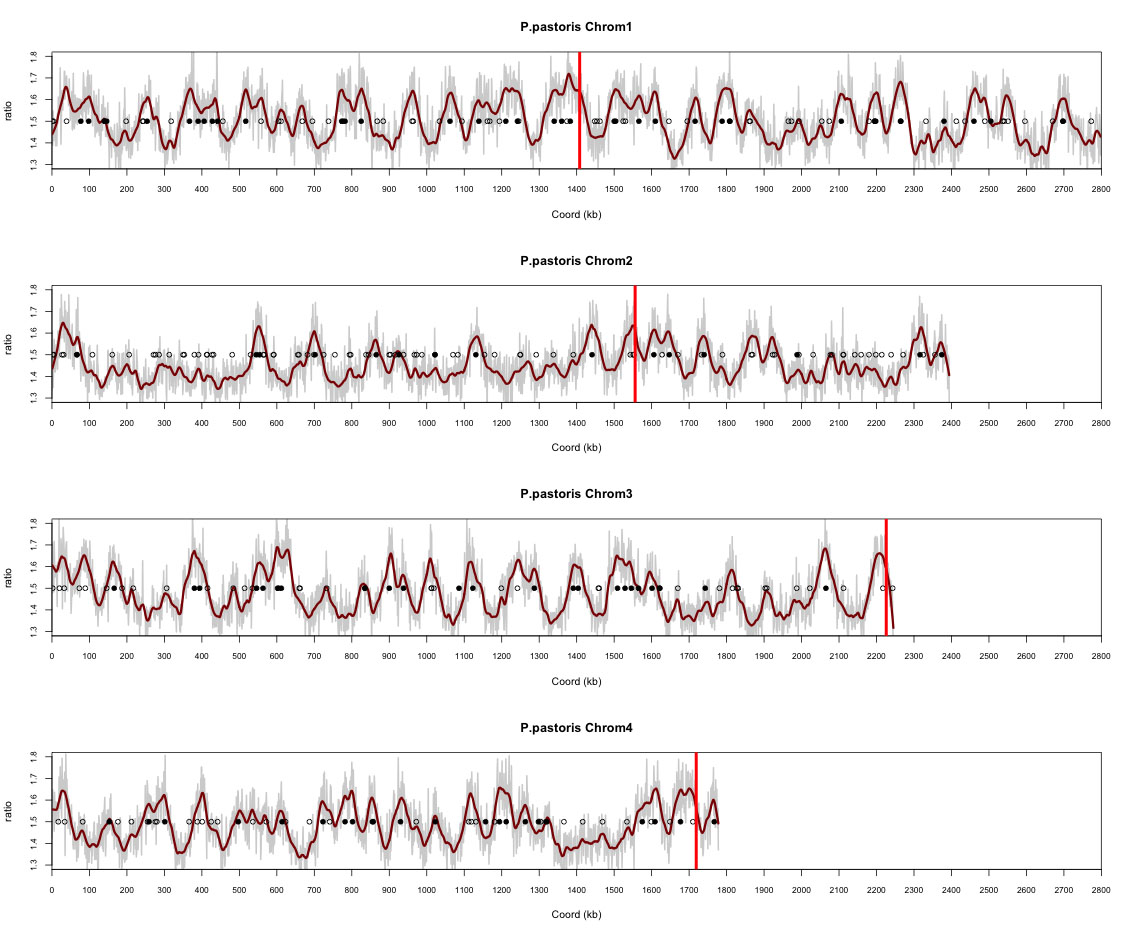
\includegraphics[width=0.9\linewidth]{figures/supp/Ppas_timing_CENs.jpg}
\label{suppfig:ppas_timing}
\end{figure}


\section*{Supplementary Notes}
%\addcontentsline{toc}{section}{Supplementary Results}

\subsection*{Initializing the optimization}
\ref{suppnotes:initialization}

The optimization problem being non convex, the local minimum found by the
algorithms depends on the starting point. We therefore implemented heuristics
to initialize the optimization with several sets of centromere positions. Our
implementation of Centurion also allows the user to specify the starting point
(\textit{ie} the rough centromere location).

For each chromosome, the centromeric regions are expected to be enriched in
\textit{trans} contact counts. We thus seek a few local maxima in the
marginalized \textit{trans} contact count profile $p(i) = \sum_{i, j |
\mathcal{B}(i) \neq \mathcal{B}(j)} c_{ij}$ for each chromosome. In order to
select only $k$ candidates per chromosome, we smooth the contact counts
profile $p$ with a Gaussian filter of parameter $\sigma$, setting $\sigma$
such that there are $k$ peaks in the profile. We consequently obtain a set of
$k$ centromere candidates per chromosome, and thus can initialize the
optimization with all possible combination of these candidates.

To reduce computation time, we implemented a set of heuristics to decrease the
number of candidates. First, note that the higher the contact count enrichment
peak is, the more likely a candidate is to be the in the centromeric region.
Second, remember that we attempt to jointly optimize centromeres location: we
optimize $L$ variables at once, $L$ being the number of chromosomes, and each
variable corresponding to a chromosome position. To reduce the number of
candidates per chromosome, we first compute a baseline, by performing the
optimization using as starting point the set of most likely candidate for each
of our $L$ chromosomes (the candidate with the highest
peak for each of the chromosomes). Then, for each candidate $p_i$ of the $l$-th
chromosome, we perform the optimization once, using as starting point the set
of most likely candidates, replacing the $l$-th one by $p_i$. If the objective
function value is higher than our baseline (thus, using $p_i$ as a candidate
for chromosome $l$ did not improved the fit), we remove the candidate from our
list. We thus reduced the number of candidates in a small number of steps and
can proceed with initializing the optimization with the all possible
combination of this reduced set of candidates. Our implementation allows the
user to specify whether or not to perform this filtering step.
